%%%%%%%%%%%%%%%%%%%%%%%%%%%%%%%%%%%%%%
% Multiplicative domain poster
% Created by Nathaniel Johnston
% August 2009
% http://www.nathanieljohnston.com/2009/08/latex-poster-template/
%%%%%%%%%%%%%%%%%%%%%%%%%%%%%%%%%%%%%%

\documentclass[final]{beamer}
\usepackage[scale=1.24]{beamerposter}
\usepackage{graphicx}			% allows us to import images
\usepackage{amsmath}
\usepackage{algorithm,algorithmicx,algpseudocode}
\usepackage[scientific-notation=true]{siunitx}

%-----------------------------------------------------------
% Custom commands that I use frequently
%-----------------------------------------------------------

\newcommand{\bb}[1]{\mathbb{#1}}
\newcommand{\cl}[1]{\mathcal{#1}}
\newcommand{\fA}{\mathfrak{A}}
\newcommand{\fB}{\mathfrak{B}}
\newcommand{\Tr}{{\rm Tr}}
\newtheorem{thm}{Theorem}

%-----------------------------------------------------------
% Define the column width and poster size
% To set effective sepwid, onecolwid and twocolwid values, first choose how many columns you want and how much separation you want between columns
% The separation I chose is 0.024 and I want 4 columns
% Then set onecolwid to be (1-(4+1)*0.024)/4 = 0.22
% Set twocolwid to be 2*onecolwid + sepwid = 0.464
%-----------------------------------------------------------

\newlength{\sepwid}
\newlength{\onecolwid}
\newlength{\twocolwid}
\setlength{\paperwidth}{48in}
\setlength{\paperheight}{36in}
\setlength{\sepwid}{0.024\paperwidth}
\setlength{\onecolwid}{0.22\paperwidth}
\setlength{\twocolwid}{0.464\paperwidth}
\setlength{\topmargin}{-0.5in}
\usetheme{confposter}
\usepackage{exscale}

%-----------------------------------------------------------
% The next part fixes a problem with figure numbering. Thanks Nishan!
% When including a figure in your poster, be sure that the commands are typed in the following order:
% \begin{figure}
% \includegraphics[...]{...}
% \caption{...}
% \end{figure}
% That is, put the \caption after the \includegraphics
%-----------------------------------------------------------

\usecaptiontemplate{
\small
\structure{\insertcaptionname~\insertcaptionnumber:}
\insertcaption}

%-----------------------------------------------------------
% Define colours (see beamerthemeconfposter.sty to change these colour definitions)
%-----------------------------------------------------------

\setbeamercolor{block title}{fg=ngreen,bg=white}
\setbeamercolor{block body}{fg=black,bg=white}
\setbeamercolor{block alerted title}{fg=white,bg=dblue!70}
\setbeamercolor{block alerted body}{fg=black,bg=dblue!10}

%-----------------------------------------------------------
% Name and authors of poster/paper/research
%-----------------------------------------------------------

\title{RNA Folding: Beyond The Thermodynamic Hypothesis}
\author{Max Ward (supervised by Amitava Datta)}
\institute{Computer Science and Software Engineering, University of Western Australia}

%-----------------------------------------------------------
% Start the poster itself
%-----------------------------------------------------------
% The \rmfamily command is used frequently throughout the poster to force a serif font to be used for the body text
% Serif font is better for small text, sans-serif font is better for headers (for readability reasons)
%-----------------------------------------------------------

\begin{document}
\begin{frame}[t]
  \begin{columns}[t]												% the [t] option aligns the column's content at the top
    \begin{column}{\sepwid}\end{column}			% empty spacer column
    \begin{column}{\onecolwid}
      
      
      \begin{block}{Introduction \& Motivation}
Ribonucleic Acid (RNA) is a biologically active molecule with many poorly understood functions. For example, it is,
\vspace{0.25in}
\begin{itemize}
\item Involved in regulation of DNA expression \\
\item Implicated in developmental pathways \\
\item A catalyst for many biological processes
\end{itemize}
\vspace{0.25in}
            
Quick and accurate prediction of RNA structure is therefore essential. RNA folding algorithms are currently not able to reliably predict correct structures. These algorithms typically globally optimize some scoring function, usually thermodynamic stability. However, there is evidence that many RNAs fold into suboptimal states.

      \end{block}
      \vskip2ex
      
      
      
      
      
      \begin{block}{My Contribution}
		        I hypothesized that local interactions are stronger than global interactions during RNA structure formation. To test this, a sliding window was used to generate locally optimal structures, then various algorithms were devised to merge these substructures. For some window sizes, the resulting complete structures were more accurate than those predicted by state of the art algorithms, which globally optimize. This constitutes strong support for my hypothesis. In addition, a new algorithm called `$ab$-splat', which was based on the computation of locally optimal windows, was introduced.
        \vspace{0.25in}
        \begin{figure}
          \begin{center}
            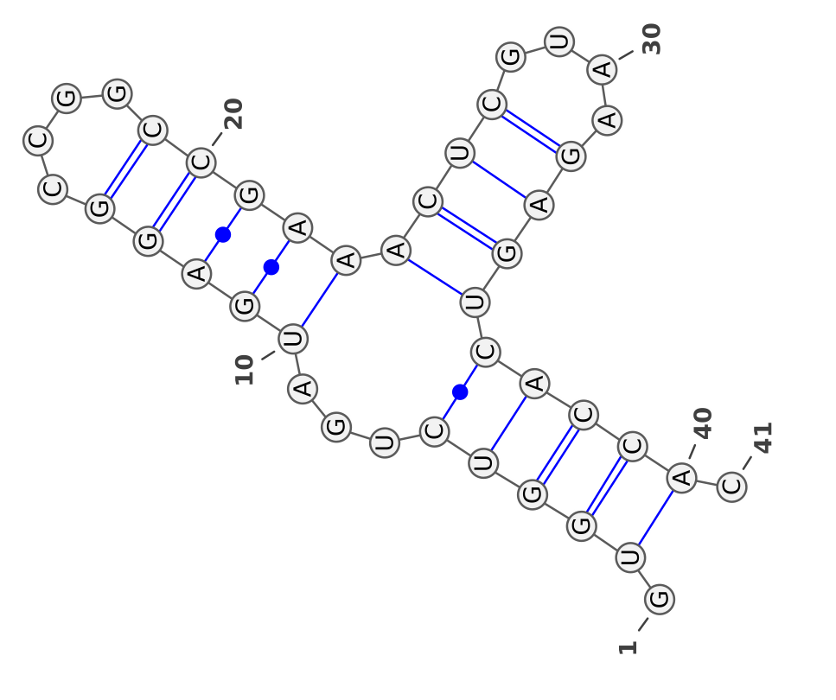
\includegraphics[width=10in]{RNAexample.png} \\
            \caption{A RNA molecule}
            \label{fig:RNAexample}
          \end{center}
        \end{figure}
      \end{block}
    \end{column}
    
    
    
    
    
    \begin{column}{\sepwid}\end{column}			% empty spacer column
    \begin{column}{\onecolwid}
    
    
    
    \begin{block}{Sliding Windows}
            Hofacker, Priwitzer, and Stadler \cite{hofacker2008rna} devised an algorithm to compute the structure of consecutive windows over a RNA in $O(nL^2)$ time, where $n$ is RNA length and $L$ is window size. This is useful when searching DNA (which can be very large) for RNA structural motifs.
\vspace{0.25in}
        \begin{figure}
          \begin{center}
            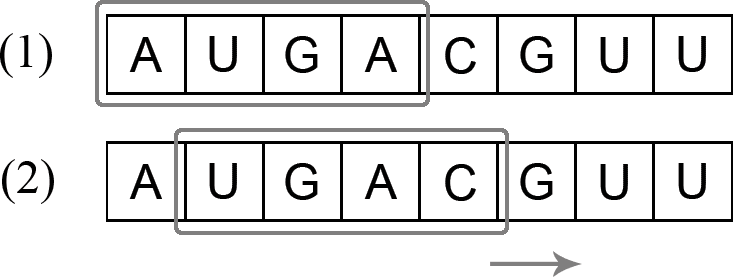
\includegraphics[width=10in]{slidingwindow.png} \\
            \caption{A sliding window over a RNA sequence}
            \label{fig:slidingwindow}
          \end{center}
        \end{figure}            
            \vspace{0.25in}
         
          \end{block}
    
     \begin{block}{Weighted Activity Selection}
The weighted activity selection problem is a classical optimization problem, and is defined as follows. Given a set of weighted intervals on a line, find a subset of intervals such that none overlap, and the sum of their weights is maximized. Such a subset can be found in $O(n \log n)$ time using dynamic programming.
\vspace{0.25in}
         
          \end{block} 
          
          
     \begin{block}{Testing Local Interactions}
To test if local interactions were stronger than global interactions, I examined window sizes 5 to 500. For every window size,

\vspace{0.25in}
\begin{itemize}
\item The sliding window algorithm was run. The structure computed for every window position was saved in a set $S$. \\
\item Every structure in the set $S$ was assigned a score. This score was defined as the free energy of the structure. The lower the free energy of a molecule, the more stable it is. \\
\item Weighed activity selection was done on the set $S$ to create a structure with minimum sum free energy.
\end{itemize}
\vspace{0.25in}
This procedure was run on a large corpus of test RNA molecules whose structure had been experimentally determined. The single most accurate prediction was recorded.

         
          \end{block} 
    
    \end{column}
    
    
    
    
    
    
 \begin{column}{\sepwid}\end{column}			% empty spacer column
    \begin{column}{\onecolwid}
    
    
    
    \begin{block}{Local Versus Global}

        \begin{figure}
          \begin{center}
            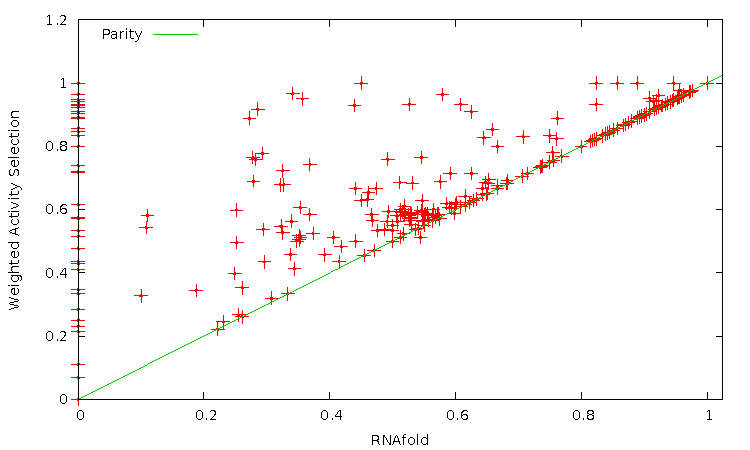
\includegraphics[width=10in]{wasrnafoldplot.pdf} \\
            \caption{Scatter plot of the best locally optimized structure, versus the prediction of RNAfold}
            \label{fig:wasvsrnafoldplot}
          \end{center}
        \end{figure}            
            \vspace{0.25in}

The Zuker algorithm, first described in 1984 \cite{someone}, is the most widely used RNA folding algorithm today. Because it has been continually refined, it is considered state of the art. In addition, the Zuker algorithm finds a structure with minimum free energy, it globally optimizes a thermodynamic scoring function. RNAfold \cite{someone} is a modern implementation of the Zuker algorithm, and was chosen for comparison.


As can be seen in Figure \ref{fig:wasvsrnafoldplot}, the procedure I described earlier was consistently more accurate than RNAfold. This result was verified by a Wilcoxon Signed-rank test ($p < 0.001$). This strongly supports my hypothesis. Because there exist window sizes for almost all tested RNA which are more accurate than the global optimum, local interactions appear to be more important than global interactions during RNA folding.
            
         
          \end{block}
    
     \begin{block}{The $ab$-splat Algorithm}
I also introduced the $ab$-splat algorithm, which is a complete RNA prediction algorithm. It utilizes locally optimal sliding windows, and weighted activity selection.
\vspace{0.25in}
        \begin{figure}
          \begin{center}
            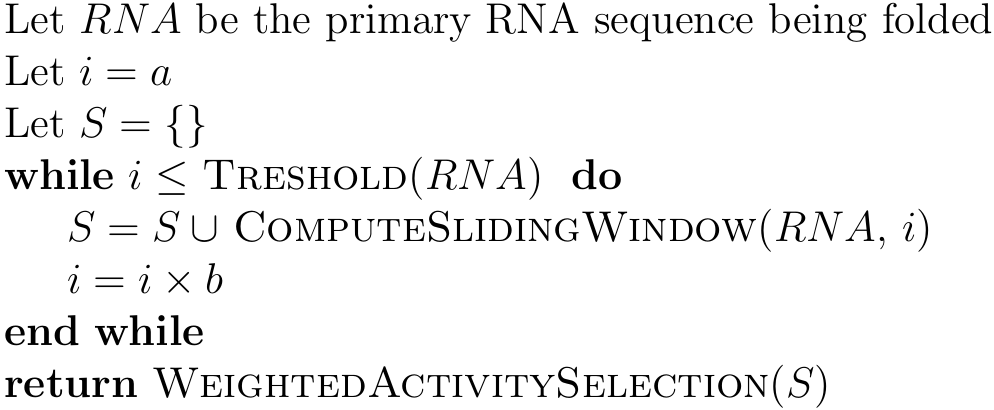
\includegraphics[width=10in]{pseudo.png} \\
            %\caption{A sliding window over a RNA sequence}
            \label{fig:psuedocode}
          \end{center}
        \end{figure}        


          \end{block} 
          
          
          
    
    \end{column}    
    
    

 \begin{column}{\sepwid}\end{column}			% empty spacer column
    \begin{column}{\onecolwid}
    
        \begin{block}{Testing $ab$-splat}


Machine learning was used to find good values ($a = blah$, $b = blah$). In addition, an effective \texttt{Threshold} function ($9.5 \times \sqrt{RNA\_Length}$) was found through empirical testing. Using this \texttt{Threshold} function, the time complexity of $ab$-splat is $O(n^2)$, where $n$ is RNA length. This is an order of magnitude faster than the Zuker algorithm, which requires $O(n^3)$ time. Again, RNAfold was used for comparison.
       \vspace{0.25in}
        \begin{figure}
          \begin{center}
            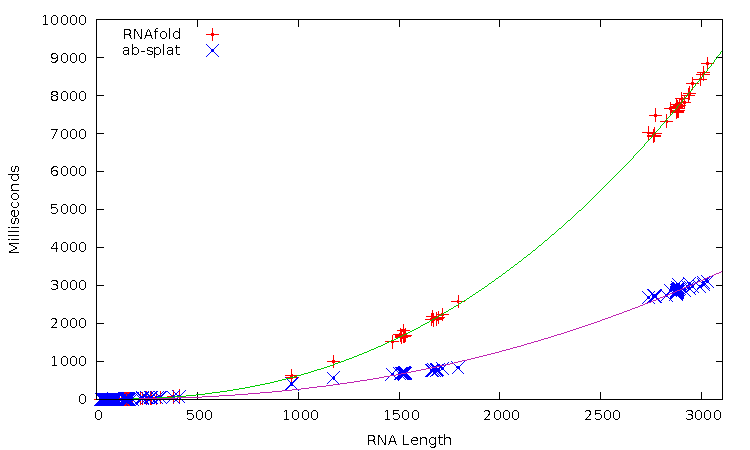
\includegraphics[width=10in]{zukerabtime.pdf} \\
            \caption{Time taken by RNAfold (red), and by $ab$-splat (blue)}
            \label{fig:zukerabtime}
          \end{center}
        \end{figure}
A Wilcoxon Signed-rank test showed that there was no statistically significant different in accuracy between RNAfold and $ab$-splat. This implies that both algorithms are equally accurate. However, the $ab$-splat algorithm was much faster in theory, and in practice (see Figure \ref{fig:zukerabtime}).   
         
          \end{block}
    
    
    \vskip2ex
    \begin{block}{References}
         
	
	\small{\begin{thebibliography}{99}
		        \bibitem{hofacker2008rna} D.~W. Kribs, R. Laflamme, D. Poulin, M. Lesosky, Quantum Inf. \& Comp. \textbf{6} (2006), 383-399.
		        \bibitem{zanardi97} P. Zanardi, M. Rasetti, Phys. Rev. Lett. \textbf{79},  3306 (1997). 
		        \end{thebibliography}}

      
      \vspace{0.5in}
      \begin{center}
          
\includegraphics[width=3in]{UWA.jpg}
      \end{center}
    \end{block}
          
          
          
    
    \end{column}    
    
    
    
    
    


        
        
  
  \begin{column}{\sepwid}\end{column}			% empty spacer column
 \end{columns}
\end{frame}
\end{document}
